\section{Musical Glossary}
\label{sec:music}

\paragraph{Pitches}
A \emph{pitch} tells us how high or low a sound is.
This notion is represented as natural numbers (of type
\texttt{Pitch}) in our implementation, with zero representing the
lowest possible sound.
Throughout the paper, we use the notation \texttt{name octave}
for pitches, where \texttt{name} ranges over \texttt{c}, \texttt{d},
\texttt{e}, etc., and \texttt{octave} denotes which octave the pitch
belongs to.
For instance, the middle C is represented as \texttt{c 5}.

% \begin{alltt}
% data Pitch : Set where
%   pitch : \(\mathbb{N}\) \(\rightarrow\) Pitch

% data Octave : Set where
%   octave : \(\mathbb{N}\) \(\rightarrow\) Octave

% PitchOctave : Set
% PitchOctave = Fin 12 \(\times\) Octave
% \end{alltt}

\paragraph{Duration}
\emph{Duration} denotes an unspecified unit of time during which
a sound or silence lasts.
In our implementation, duration is again a natural number (of type
\texttt{Duration}), with names such as \texttt{whole}, \texttt{half},
and \texttt{quarter}.
These values are turned into an absolute length when the music is
played at a specific tempo.
As an example, \texttt{whole} has value \texttt{16} and corresponds
to 4 seconds if the tempo is 60 beats per minute.

% \begin{alltt}
% data Duration : Set where
%   duration : \(\mathbb{N}\) \(\rightarrow\) Duration
% \end{alltt}

\paragraph{Notes}
Combining pitches and duration gives us \emph{notes}.
We construct notes (of type \texttt{Note}) with the \texttt{tone}
and \texttt{rest} constructors.
For example, \texttt{tone whole (c 5)} is a whole note whose
sound is the middle C, and \texttt{rest half} is a half rest.

% \begin{alltt}
% data Note : Set where
%   tone : Duration \(\rightarrow\) Pitch \(\rightarrow\) Note
%   rest : Duration         \(\rightarrow\) Note
% \end{alltt}

\paragraph{Intervals}

An \emph{interval} represents the difference in pitch between
two notes.
There are 13 kinds of interval within an octave, and these
intervals can be classified from several different perspectives:
(i) major or minor; (ii) consonant or dissonant; and (iii) perfect
or imperfect.
We define intervals as a datatype \texttt{Interval}, where each
constructor represents one of the 13 intervals.

\begin{figure}[h]
  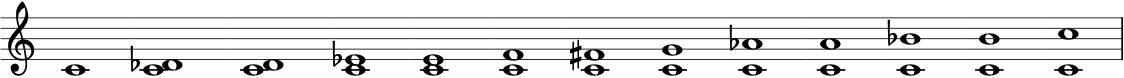
\includegraphics[width=12cm]{fig/interval.png} \\
  \begin{flushleft}
    \begin{footnotesize}
      \hspace{1.45cm} \texttt{per1 \hspace{0.5mm} min2  \hspace{2.5mm}
        maj2 \hspace{1.2mm} min3 \hspace{0.5mm} maj3 \ per4
        \hspace{1mm}aug4
        \hspace{0.5mm}  per5\hspace{1.2mm}  min6\hspace{1.6mm} maj6
        \hspace{1.6mm}min7\hspace{1.2mm} maj7\hspace{1.2mm} per8} \\
      consonant? \hspace{1.5mm} yes \hspace{4.2mm} no \hspace{6.5mm}  no
      \hspace{4.7mm} yes \hspace{3.8mm}  yes \hspace{3.7mm} no \hspace{3.5mm}
      no \hspace{4.3mm} yes \hspace{3.8mm} yes \hspace{3.2mm} yes
      \hspace{3.7mm} no \hspace{4mm} no \hspace{3.8mm} yes
    \end{footnotesize}
  \end{flushleft}
\end{figure}